\chapter{Sketching in 3D}

In a 2-D sketching application on a graphical tablet, a user draws on a two dimensional plane that mirrors the surface of the input device.
However, in a 3-D sketching application, the user draws curves on arbitrary three dimensional planes and objects.
The most basic example is a simple plane: a user can orient a plane in three dimensional space, and the draw on the tablet.
The strokes on the tablet are then projected onto the plane, thereby creating a 3-D stroke.

A similar technique exists in rendering algorithms in computer graphics, called ray tracing.
Ray tracing is primarily used for the creation of realistic images; it determines visible surfaces at the pixel level. 
Starting at points on the lens of a virtual camera, rays are sent into an environment until they intersect with geometry.
In between the environment and the camera is a virtual image plane, a grid representing the pixels of the final image.
Where a ray intersects with the image plane determines what pixel the ray effects.
A subset of this algorithm can be used to solve for the stroke projection onto a virtual drawing object, the ray casting algorithm.


\begin{figure}
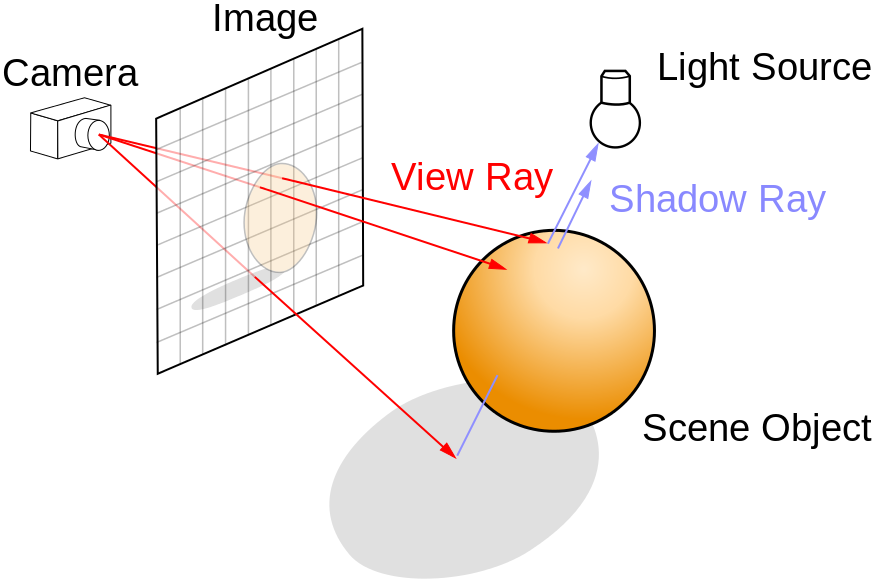
\includegraphics[width=0.9\linewidth]{raytracediagram}
\caption{Ray Tracing in Computer Graphics}
\end{figure} 
\begin{figure}
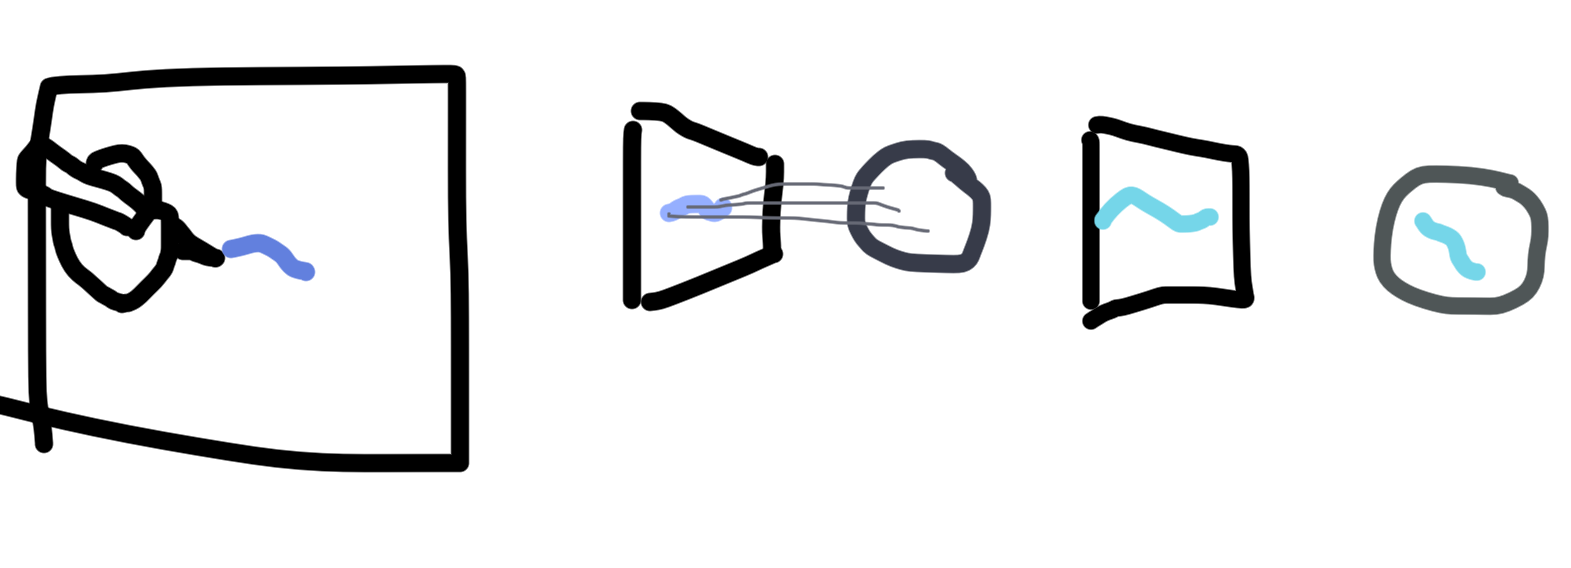
\includegraphics[width=0.9\linewidth]{StrokeProjection}
\caption{Rough Diagram of Projecting Stroke onto Drawing Surface}
\end{figure} 

\section{Ray Casting}

Ray casting is the use of rays, a line with an endpoint and a direction, to test for intersections with surface geometry.
These computations are the fundamentals of ray tracing computer graphics algorithms, used to solve a variety of problems.

A common use of ray casting is object selection in an interactive 3-D application.
The mouse is clicked in pixel $(i,j)$, and the "picked" object is whatever is "seen" though the pixel.
Using ray casting, a ray is created at pixel $(i,j)$ and sent in the virtual viewing direction.
If it intersects, then the object at the point of intersection is selected.
Through this example, we can see a method of using ray casting in order to project a stroke into the virtual space.
The ray casting algorithm is utilized as follows:
\begin{itemize}
\item The user draws a stroke on a 2-D plane, giving a set of sample points
\item An imaginary plane is created in the virtual space representing the image plane.
\item Rays are cast into the three dimensional scene from the imaginary plane based on the sample positions.
\item The intersections with scene geometry represent the new 3-D positions of the stroke
\end{itemize}
Once we intersect all of the sample points with the scene geometry, we can use the spline techniques described in the previous chapter to create a 3-D curve approximating the appearance of the projected 2D stroke.

\subsection{Generating the Ray}

A ray is mathematically defined as an origin point and a movement direction, usually represented as a parametric line.
The ray is generated in the same way view rays are created in ray tracing; assuming we have an eye $\mathbf{e}$ and a point on the screen plane $\mathbf{s}$, the line is defined by:
\begin{equation}
p(t) = \mathbf{e} + t(\mathbf{s} - \mathbf{e})
\end{equation}
Given a value $t$, we can determine any point that lies along the line, with $p(0) = \mathbf{e} \text{ and } p(1) = \mathbf{s}$.
For positive values of $t$, if $t_1 < t_2$, then $t_1$ is closer to the eye than $t_2$, and if $t < 0$, then the point is behind the ray.
\begin{figure}
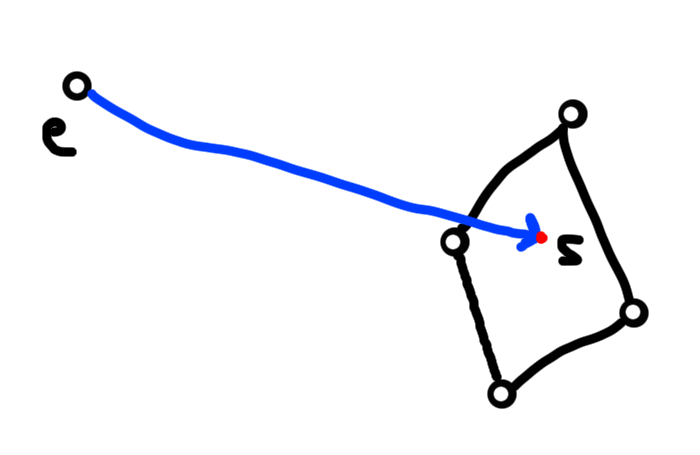
\includegraphics{etos}
\caption{The ray from the eye $\mathbf{e}$ to a point on the screen $s$}
\end{figure}

Computing a ray means solving for $s$ using the relative coordinate axis of the camera, the aspect ratio of the display, and a pixel position $(i,j)$.
$s$ is calculated as follows:
\begin{itemize}
\item Moving from the eye to the view plane by using a defined distance for the near plane ($w_s$) and the forward view direction ($\mathbf{w}$) of the camera
\item Calculate the a $u_sv_s$ coordinate on the view plane based on the pixel $(i,j$).
\item Move $u_s$ units in the camera's right direction ($\mathbf{u}$), and $v_s$ units in the up direction ($\mathbf{v}$).
\end{itemize}
This process can be expressed as:
\begin{equation}
\mathbf{s} = \mathbf{e} + u_s\mathbf{u} +v_s\mathbf{v}+w_s\mathbf{w}.
\end{equation}


\subsection{Ray-Triangle Intersection}

Given a ray $\mathbf{e} + t\mathbf{d}$, where $\mathbf{e}$ is the origin of the ray and $\mathbf{d}$ is the direction, we want to find the first intersection with any object where $t > 0$.
In this section, the intersection the most basic computer graphics primitive, the triangle, is discussed.
Any object in a real-time computer graphics application is constructed or approximated using triangles, including curved surfaces such as spheres.
Thus, being able to intersect with a single triangle will allow 3D sketching on any object used for the application.

For our algorithm, we will intersect a ray with a parametric plane that contains the triangle.
Once intersected, we use barycentric coordinates to check if the intersection point is contained within the boundaries of the triangle. 
Note we could eliminate this check if we want to draw on an infinite intersection plane.
This method requires only the vertices of the triangle.

To intersect a ray with a parametric surface, a system of equations is created where the Cartesian coordinates all match:
\begin{align}
x_o + tx_d = f(u,v) \\
y_o + ty_d = g(u,v) \\
z_o + tz_d = h(u,v)
\end{align}
Here there are three equations and three unknowns ($t$, $u$, and $v$).
When a parametric surface is a parametric plane, the parametric equation can be written in vector form.
If the vertices of the triangle are $\mathbf{a}$, $\mathbf{b}$, and $\mathbf{c}$, then the intersection occurs when
\begin{align}
\mathbf{e} + t\mathbf{d} = \mathbf{a} + \beta(\mathbf{c}-\mathbf{a}) + \gamma(\mathbf{c}-\mathbf{a}).
\end{align}
$\beta$ and $\gamma$ are two of the three barycentric coordinates of the triangle. 
If $\beta > 0, \gamma > 0,$ and $\beta + \gamma < 1$, then the intersection point lies inside of the triangle; otherwise it hits the plane outside the triangle.
If there are no solutions, then either the triangle is degenerate or the ray is parallel to the parametric plane.

To solve for $t, \beta, \text{and} \gamma$, equation 1.4 is expanded from the vector form to equations for each of the three coordinate planes.
\begin{align}
x_o + tx_d = x_a + \beta(x_b-x_a) + \gamma(x_c-x_a) \\
y_o + ty_d = y_a + \beta(y_b-y_a) + \gamma(y_c-y_a) \\
z_o + tz_d = z_a + \beta(z_b-z_a) + \gamma(z_c-z_a)
\end{align}
This can be rewritten into a standard linear equation of the form $Ax = b$:
\begin{align}
\begin{bmatrix}
x_a - x_b & x_a - x_c & x_d \\
y_a - y_b & y_a - y_c & y_d \\
z_a - z_b & z_a - z_c & z_d
\end{bmatrix}
\begin{bmatrix}
\beta \\ \gamma \\ t
\end{bmatrix}
= \begin{bmatrix}
x_a - x_o \\ y_a - y_o \\ z_a - z_o
\end{bmatrix}
\end{align}
This can be solved using Cramer's rule: given a system of $n$ linear equations for $n$ unknowns, represented as $Ax = b$, where the $n \times n$ matrix $A$ has a nonzero determinant, and the vector $x = (x_1, \ldots, x_n)^\mathrm{T}$ is the column vector of the variables, the system has a unique solution.
This solution is given by
\begin{equation}
x_i = \frac{\det(A_i)}{\det(A)} \qquad i = 1, \ldots, n
\end{equation}
where  $A_i$  is the matrix formed by replacing the $i$-th column of $A$ by the column vector $b$.
Solving gives the solutions:
\begin{align}
\beta = \frac{\begin{vmatrix}
x_a - x_o & x_a - x_c & x_d \\
y_a - y_o & y_a - y_c & y_d \\
z_a - z_o & z_a - z_c & z_d
\end{vmatrix}}{|A|} \\
\gamma = \frac{\begin{vmatrix}
x_a - x_b & x_a - x_o & x_d \\
y_a - y_b & y_a - y_o & y_d \\
z_a - z_b & z_a - z_o & z_d
\end{vmatrix}}{|A|} \\
t = \frac{\begin{vmatrix}
x_a - x_b & x_a - x_c & x_a - x_o \\
y_a - y_b & y_a - y_c & y_a - y_o \\
z_a - z_b & z_a - z_c & z_a - z_o
\end{vmatrix}}{|A|} 
\end{align}
where A is given in equation 1.8, and $|A|$ denotes the determinant of $A$.

\section{Acceleration Structures}

An acceleration structure must be used in order to give sub-linear time for ray object intersection for complex objects.
In a naive implementation, the ray caster would iterate over all triangles in the scene to check for intersections, giving $O(N)$ performance.
For sufficiently large values of $N$, this would be very slow, thus a "divide and conquer" algorithmic approach is used, creating an ordered data structure to speed up the intersection process.

While many approaches exist, this project implements a simple bounding volume hierarchy (BVH) tree (Rubin \& Whitted, 1980).

\subsection{Bounding Boxes}

A bounding box for a point set $S$ in $N$ dimensions is the box with the smallest measure (area, volume, or hypervolume) within which all the points lie.
For this project, we use axis-alligned bounding boxes (AABBs), which are constrained so their edges lie parallel to the Cartesian coordinate axis.
A key operation in any intersection acceleration structure is computing the intersection of a ray and a bounding box.
For this, it is not necessary to calculate where the ray hits the box, only if it is hit at all, as the box itself is a final piece of geometry.

The fastest method for intersecting a ray with an AABB is the slab method.
The idea is to treat the bounding box as the space contained inside of $N$ pairs of parallel planes.
For each pair of planes, two pairs of $t$ values, $t_min$ and $t_max$ are solved for the segment that is between the two planes.
If the largest $t_min$ is smaller than the smallest $t_max$, then some portion of the ray is contained within all three planes.

\begin{figure}
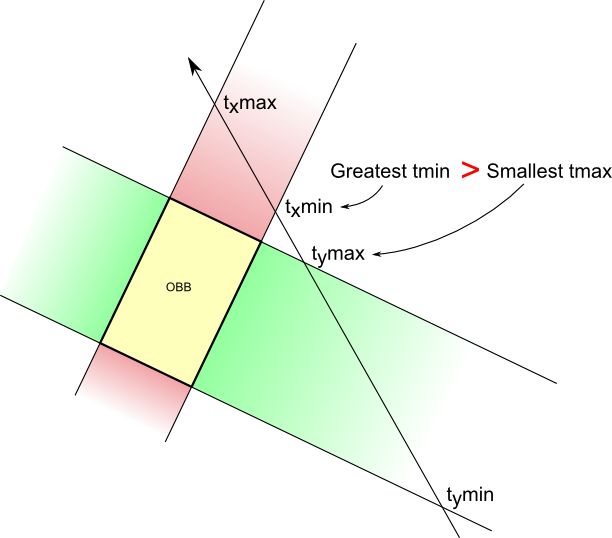
\includegraphics{AABBray}
\caption{An example of a ray checking and failing for intersection with a box}
\end{figure}

\subsection{BVH Tree}
 A bounding volume hierarchy (BVH) is a tree data structure on a set of geometric objects.
 All objects are wrapped in bounding volumes that form the leaf nodes of the tree.
 These nodes are then grouped into small sets and enclosed within larger bounding volumes.
 This grouping occurs recursively until there is a single bounding volume at the top of the tree.
 By using this data structure, the complexity of the a ray cast on a complex scene can be reduced from linear based on the number of objects to logarithmic.
 
 A good BVH tree has the following properties:
 \begin{itemize}
 \item The nodes in a given sub tree should be close to each other. The lower down the tree, the closer the nodes should be.
 \item Each node in the BVH should be of minimum volume.
 \item The sum of all bounding volumes should be minimized.
 \item The volume of overlap of sibling nodes should be minimized.
 \item The BVH should be balanced with respect to both its node structure and its content. Balancing allows as much of the BVH to be pruned when not traversed.
 \end{itemize}
Because of the number of properties a good BVH tree has, a good algorithm must be used for constructing the tree.
The current bast algorithm is the Surface Area Heuristic (SAH).
The idea behind SAH is to balance both the number of objects contained in a bounding volume while minimizing the surface area of the volume itself.
This is an exceptionally slow heuristic, so while providing the fastest solution at runtime, the construction cost must be considered for use in real time applications.

\paragraph{Basic BVH Algorithm}
\begin{enumerate}
\item Decide on a cost function that will check the quality of your object division
\item Create Bounding Box for current Node.
\item Sort along all 3 axis and find the axis with the best cost, and find the object position that will be your center.
\item Divide the objects.
\end{enumerate}

\begin{figure}
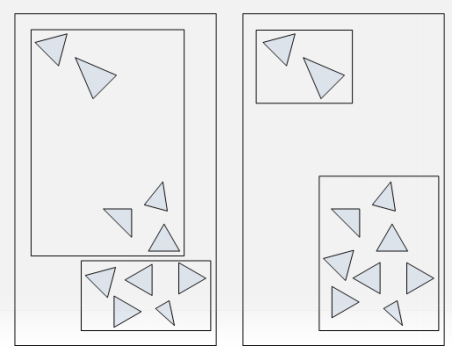
\includegraphics[width=\textwidth]{sahbvh}
\caption{A comparison between the bounding volumes of a node using a naive implementation (left) and a surface area heuristic (right).}
\end{figure}